\documentclass{beamer}
\usetheme{Madrid}
\usepackage{lmodern}% http://ctan.org/pkg/lm
\setbeamersize{text margin left = 2.5em}
\setbeamersize{text margin right = 2.5em}
\usepackage{color}
\usepackage{graphicx}
\usepackage{MnSymbol}
\usepackage{amsmath}
\usepackage{comment}
\usepackage{tikz}
\usepackage{subfigure}
\usepackage{listings}
\usetikzlibrary{automata}

%\usepackage[backend=bibtex,sorting=none]{biblatex}
%\addbibresource{E:/Papers/LiuLab} %BibTeX�����ļ���λ��
%\setbeamerfont{footnote}{size=\tiny}
\setbeamertemplate{theorems}[numbered]
\setbeamertemplate{caption}[numbered]
%% ʹ�ý�ע���õ�Ƭijҳ���Ӳο����ס�
%% ��������ʹ�ã�\footfullcite{bib_item} %����item
%% \usepackage{anyfontsize}%% allowing font sizes at arbitrary sizes
\logo{
\includegraphics[height=0.05\textwidth]{Pic/logo}}
\newtheorem{df}{Definition}
\newtheorem{DF}{DEFINITION}
\newtheorem{prop}{Proposition}
\newtheorem{thm}{Theorem}
\newtheorem{cor}{COROLLARY}
\newtheorem{lm}{LEMMA}
% ----------------------------------------------------------------------------------------
% TITLE PAGE
% ----------------------------------------------------------------------------------------

\title{E03 Othello Game}
% The short title appears at the bottom of every slide, the full title is only on the title page

\author{Suixin Ou} % Your name
\institute[SYSU] % Your institution as it will appear on the bottom of every slide, may be shorthand to save space
{
  School of Computer Science\\
  Sun Yat-sen University \\ % Your institution for the title page
  \medskip
  % Your email address
}

\date{September 28, 2021} % Date, can be changed to a custom date

\AtBeginSection[]
{
  \begin{frame}
    \tableofcontents[currentsection,currentsubsection]
  \end{frame}
}

\begin{document}

\begin{frame}
  \titlepage
\end{frame}

\begin{frame}
  \frametitle{Task}
  \begin{block}{Problem}
    Othello (or Reversi) is a strategy board game for two players, played on an 6 $\times$ 6 uncheckered board.

    \begin{figure}[ht]
      \centering
      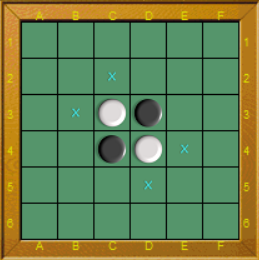
\includegraphics[width=0.3\textwidth]{Pic/2thello}
      \caption{Othello Game}
    \end{figure}
  \end{block}
\end{frame}

\begin{frame}
  \frametitle{Task}
  \begin{block}{Problem}
During a play, any disks of the opponent's color that are in a straight line and bounded by the disk just placed and another disk of the current player's color are turned over to the current player's color.

    \begin{figure}[ht]
      \centering
      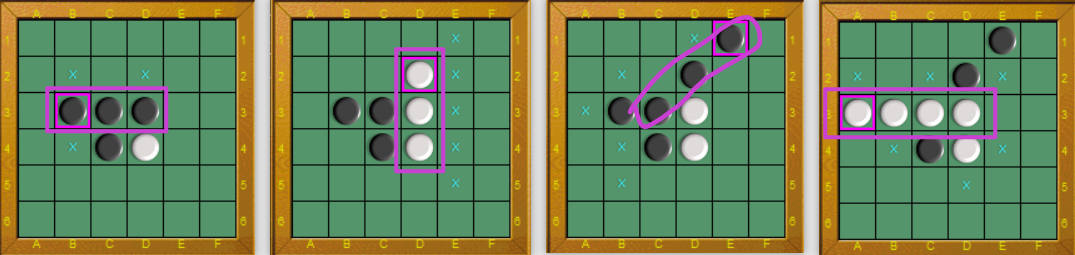
\includegraphics[width=1.0\textwidth]{Pic/2thello1}
      \caption{Take a turn}
    \end{figure}
  \end{block}
\end{frame}

\begin{frame}
  \frametitle{Task}
  \begin{block}{Description}
    \begin{itemize}
      \item Choose an appropriate evaluation function and use min-max and $\alpha - \beta$ prunning to implement the Othello game. The framework file you can refer to is Othello.cpp. 
\item I wish you to compare the performance of different heuristic evaluation functions (by comparing chess skills of different agents). 
\item Further more, you are also encouraged to compare the efficiency of minimax and $\alpha - \beta$ prunning algorithm.
	  \item There are several evaluation functions that involve many aspects, you can turn to http://www.cs.cornell.edu/~yuli/othello/othello.html for help.
    \end{itemize}
  \end{block}
\end{frame}

\begin{frame}
  \frametitle{Solution}
The $\alpha - \beta$ pruning algorithm that will be used in this exercise is in line 59:

    \begin{figure}[ht]
      \centering
      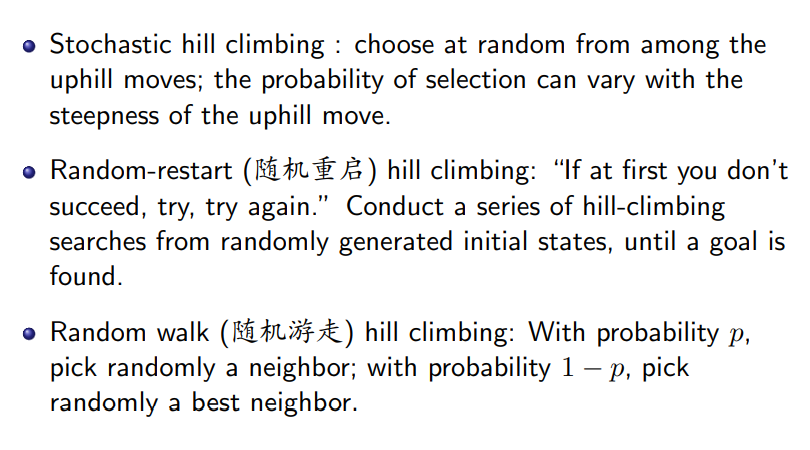
\includegraphics[width=1.0\textwidth]{Pic/algorithm}
    \end{figure}

	We already provide a naive evaluation function in Othello.cpp, which should be exceeded by better ones.
    \begin{figure}[ht]
      \centering
      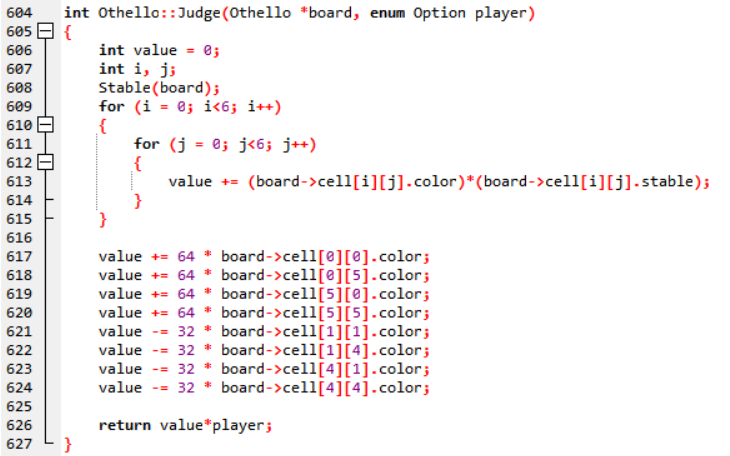
\includegraphics[width=1.0\textwidth]{Pic/evalfunc}
    \end{figure}
\end{frame}

\begin{frame}
  \begin{block}{Submission}
    pack your report \texttt{E03\_YourNumber.pdf} and source code into zip file \texttt{E03\_YourNumber.zip}, then send it to \texttt{ai\_course2021@163.com}.
  \end{block}
\end{frame}

%-----------------------------------------------------------------------------------------

\begin{frame}
  \Huge{\centerline{The End}}
\end{frame}

% ----------------------------------------------------------------------------------------


\end{document}
